\documentclass[conference, a4paper]{IEEEtran}
\usepackage{blindtext, graphicx, url}
\hyphenation{}


 %%% JS %%%
%Define the listing package
\usepackage{listings} %code highlighter
\usepackage{color} %use color
\definecolor{mygreen}{rgb}{0,0.6,0}
\definecolor{mygray}{rgb}{0.5,0.5,0.5}
\definecolor{mymauve}{rgb}{0.58,0,0.82}

%Customize a bit the look
\lstset{ %
backgroundcolor=\color{white}, % choose the background color; you must add \usepackage{color} or \usepackage{xcolor}
basicstyle=\footnotesize, % the size of the fonts that are used for the code
breakatwhitespace=false, % sets if automatic breaks should only happen at whitespace
breaklines=true, % sets automatic line breaking
captionpos=b, % sets the caption-position to bottom
commentstyle=\color{mygreen}, % comment style
deletekeywords={...}, % if you want to delete keywords from the given language
escapeinside={\%*}{*)}, % if you want to add LaTeX within your code
extendedchars=true, % lets you use non-ASCII characters; for 8-bits encodings only, does not work with UTF-8
frame=single, % adds a frame around the code
keepspaces=true, % keeps spaces in text, useful for keeping indentation of code (possibly needs columns=flexible)
keywordstyle=\color{blue}, % keyword style
% language=Octave, % the language of the code
morekeywords={*,...}, % if you want to add more keywords to the set
rulecolor=\color{black}, % if not set, the frame-color may be changed on line-breaks within not-black text (e.g. comments (green here))
showspaces=false, % show spaces everywhere adding particular underscores; it overrides 'showstringspaces'
showstringspaces=false, % underline spaces within strings only
showtabs=false, % show tabs within strings adding particular underscores
% stepnumber=1, % the step between two line-numbers. If it's 1, each line will be numbered
stringstyle=\color{mymauve}, % string literal style
tabsize=2, % sets default tabsize to 2 spaces
title=\lstname % show the filename of files included with \lstinputlisting; also try caption instead of title
}
%END of listing package%

\definecolor{darkgray}{rgb}{.4,.4,.4}
\definecolor{purple}{rgb}{0.65, 0.12, 0.82}

%define Javascript language
\lstdefinelanguage{JavaScript}{
keywords={typeof, new, catch, function, return, null, catch, switch, var, if, in, while, do, else, case, break, for},
keywordstyle=\color{blue}\bfseries,
ndkeywords={class, export, boolean, throw, implements, import, this, true, false, Math},
ndkeywordstyle=\color{darkgray}\bfseries,
identifierstyle=\color{black},
sensitive=false,
comment=[l]{//},
morecomment=[s]{/*}{*/},
commentstyle=\color{purple}\ttfamily,
stringstyle=\color{red}\ttfamily,
morestring=[b]',
morestring=[b]"
}

\lstset{
language=JavaScript,
extendedchars=true,
basicstyle=\ttfamily,
showstringspaces=false,
showspaces=false,
tabsize=2,
breaklines=true,
showtabs=false,
captionpos=b
}

 %%% END JS %%%


\begin{document}
\title{How does the implementation of\\
Strategy Design Pattern in JavaScript\\
affect Maintainability as measured by Cyclomatic Complexity and Lines of Code}
\author{\IEEEauthorblockN{Oskar Ther\'{e}n}
\IEEEauthorblockA{Computer Engineering\\
The Institute of Technology at Link\"{o}ping University\\
Email: oskth878@student.liu.se}}

\maketitle

\begin{abstract}
	 In this paper an implementation of the Strategy Design Pattern, as originally described in the book ``Design Patterns: Elements of Reusable Object-Oriented Software'', is presented in the high-level and untyped programming language JavaScript. It is implemented in an existing game, where it replaces a switch statement to reduce Cyclomatic Complexity. The difference in Cyclomatic Complexity and Lines of Code before and after the implementation is evaluated in the aspect of how it affects maintainability. This paper is concluded with some discussion about the usefulness of implementing the pattern in a bigger project.
\end{abstract}

\section{Introduction}
\label{sec:Introduction}
It is widely acknowledged in object-oriented programming that Design Patterns can be useful for solving commonly occurring problems within a given context  by creating reusable code. Design Patterns were mainly introduced to software developers through the GoF (Gang of Four) that wrote about the concept in their book, ``Design Patterns: Elements of Reusable Object-Oriented Software''~\cite{bibitem:GoF}, though the idea originally comes from an architectural concept. The patterns have since been widely discussed, customized and used.

The Design Patterns are created from an object oriented perspective, while on the other hand web development is most commonly conducted in the dynamic, untyped and interpreted language JavaScript. More and more businesses are moving their products over to the web and with that comes high expectations on code quality. Harmes et al.~\cite{bibitem:DiazHarmes} and Osmani~\cite{bibitem:Osmani} have proposed to adapt the GoF's Design Patterns to make them applicable to JavaScript, in an attempt to make the code safer, more reusable and easier to maintain.

When using Design Patterns it might not always be good to follow them blindly. Zhang et al. argues in their article ``What Do We Know about the Effectiveness of Software Design Patterns?'' that even though Design Patterns are so popular, there are few empirically justified reasons to use them.~\cite{bibitem:Zhang}

The purpose of this paper is to find out if the implementation of a specific Design Pattern, will affect maintainability in a positive way, measured by two metrics in the programming language JavaScript. All of these concepts are in depth explained in the Background of this paper section~\ref{sec:Background}.

\subsection{Research Question}
\begin{itemize}
	\item How does the implementation of Strategy Design Pattern in JavaScript affect Maintainability as measured by Cyclomatic Complexity and Lines of Code?
\end{itemize}

\section{Background}
\label{sec:Background}

\subsection{Strategy Design Pattern}
\label{sec:Strategy}

Strategy is a behavioral pattern that is created to minimize coupling by encapsulating a family of algorithms and make them interchangeable by abstracting away the algorithms' different functionalities into separate classes that implement a common interface, which is called strategy. An UML diagram of the concept is shown in Figure \ref{fig:Strategy}. For a language to be able to implement Strategy in the way it is explained by the GoF it needs something similar to a Java interface. JavaScript does not have the concept of interface, which is further discussed in section~\ref{sec:JavaScript}.~\cite{bibitem:GoF}

\begin{figure}[ht!]
	\centering
	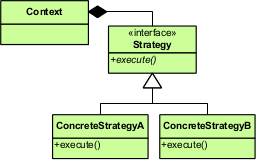
\includegraphics[scale=0.7]{Strategy_Pattern_in_UML.png}
	\caption{Strategy Pattern in a UML diagram.}
	\label{fig:Strategy}
\end{figure}

The GoF claims that one of the main applications of the pattern is to put conditional branches into new classes they call Strategy classes when there several conditionals with many behaviors~\cite{bibitem:GoF}. This is motivativation that the example used in this paper, Listing~\ref{lst:switch-case}, is a good starting point.

When discussing Design Patterns it is important to note that is not always a perfect solution and have received some criticism. Zhang et al. is critical to the fact that some Design Patterns benefits are supported by weak empirical evidence.~\cite{bibitem:Zhang}

``The Difficulties of Using Design Patterns among Novices: An Exploratory Study'' by Abdul Jalil et al. explores novice programmers' difficulties when applying Design Patterns. Their conclusion on the Strategy Pattern is that it is not so hard to understand nor apply. This study says nothing about the actual effect on the code.~\cite{bibitem:Jalil}

Khomh et al. wanted to empirically evaluate how some software qualities are affected by design patterns. They showed that some patterns generally  have negative impact on some quality attributes. The Strategy Pattern did according to their study have a positive impact on some aspects such as simplicity, modularity, learnability and understandability, all important attributes relating to maintainability. On the other hand they showed results of negative impact on reusability and robustness.~\cite{bibitem:DPaSQ}

\subsection{SOLID}
The purpose of many Design Patterns is to solve some of the SOLID-violations that can arise when working on bigger projects. SOLID is an mnemonic acronym that stands for
\begin{itemize}
    \item \emph{Single responsibility} \\
    Each class should only have responsibility over one part of the software's functionality.
    \item \emph{Open-closed} \\
    Classes, functions and so on, should be open for extension but closed for modification.
    \item \emph{Liskov substitution} \\
    Every subtype should be able to replace its inherited type.
    \item \emph{Interface segregation} \\
    Clients should not be forced to implement methods from an interface that it will not use.
    \item \emph{Dependency inversion} \\
    High level modules should not be affected by changes of low level modules.
\end{itemize}

These principles were developed by RC Martin in his books about Agile development but they can be applicable to a lot of different aspects of software development. They are generally good to follow when developing software and are all contributing to code that is for example easier to maintain.~\cite{bibitem:Bob}

The Strategy Pattern mainly improves the code with Single responsibility and Open-closed in aspect, although it follows the other principles as well:

\textit{Single Responsibility} through having the code for the algorithms in separate classes.

\textit{Open-closed} because when a new algorithm is introduced, the existing code will not have to be changed. Though a new class for that algorithm needs to be added to extend the interface.

\subsection{Design Patterns in JavaScript}
There are some attempts of using Design Patterns in JavaScript, with different levels of modification. In the book ``Pro JavaScript\texttrademark~Design Patterns'' from Harmes et al. they try to create GoF's book for JavaScript developers which they motivates with the following reasons:
\begin{itemize}
    \item \emph{Maintainability} \\
		Makes modules less coupled which makes refactoring easier.
    \item \emph{Communication} \\
		Easier to discuss the code on a higher level with other developers.
    \item \emph{Performance} \\
    Some patterns can improve the performance of the program.
\end{itemize}
They also mention some drawbacks with Design Patterns, some of them can have a negative performance impact while others can make the code more complex and harder to understand by newer developers.~\cite{bibitem:DiazHarmes}

Another book on the subject is Osmanis ``Learning JavaScript Design Patterns: A JavaScript and jQuery Developer's Guide'' which provides his interpretation of some of the GoF's Design Patterns both for JavaScript and the library jQuery. He discusses the different patterns and their usefulness in JavaScript.~\cite{bibitem:Osmani}

Both books contains arguments on why Design Patterns can be useful in JavaScript but neither implements the Strategy Pattern. There is no obvious reason for this since the Strategy Pattern can be applied to remove the use of multiple conditionals, as mentioned in section~\ref{sec:Strategy}, which is as relevant in JavaScript as in object oriented languages. That makes the pattern an interesting choice for this paper.

\subsection{Maintainability and Metrics}
\label{sec:Maintainability}

Since the 1991 when the ISO standard for maintainability was introduced (ISO 9126) there have been several attempts to link maintainability with different metrics. Heitlager et al. argues that a problem with the standard is that the suggested maintainability metrics measure the wrong things. They focus on the technical staffs maintenance performance instead of measuring the systems source code.~\cite{bibitem:Maintainability}

There are several metrics that try to measure the complexity of a function or a program. These metrics have different advancement levels, they range from easily measured metrics like Lines of Code or Cyclomatic Complexity to Robillards interconnectivity metric that ``integrates the structural as well as the textual aspects of a program in such a way that the organization of a program can be seen graphically. The measure of complexity depends on how a statement is related to the rest of the program.''~\cite{bibitem:Robillard}

In the paper ``Using Metrics to Evaluate Software System Maintainability'', Coleman et al. found that when they conducted automated software maintainability analysis on 11 software systems, they all corresponded to the experts' intuition and also provided additional useful data. The metric they created is widely used by among others Visual Studio by Microsoft~\cite{bibitem:MI}. It is called MI (Maintainability Index) which is calculated as a factored formula consisting of Source Lines of Code, Cyclomatic Complexity, Halstead Volume and percent of Lines of Comments. Where Halstead Volume is calculated from the programs lenght, amount of operands and amount of operators.~\cite{bibitem:MetricsToEvaluate}


Heitlage et al. discusses several problems with MI, which are summarized below:
\begin{itemize}
    \item \emph{Root-cause analysis} \\
    Since the formula just gives a number it can be hard to know what the cause of a bad value is.
    \item \emph{Average complexity} \\
    This value will be small even though some methods might have high complexity, since most methods will not. They argue that an average value in this case is misleading.
    \item \emph{Computability} \\
		The Halstead Volume is difficult to define and compute.
    \item \emph{Comment} \\
		Comments have no correlation with maintainability at all in general.
    \item \emph{Understandability} \\
		The formula is hard to understand since it for example contains several constants that are introduced without any logical arguments.
		\item \emph{Control} \\
		The developers and management can easily feel a lack of control over the MI value.
\end{itemize}
They move on to suggest a metric of their own that is also using Lines of Code and Cyclomatic Complexity. They argue that it is better to calculate Cyclomatic Complexity per unit, where a unit is the smallest piece of code that can be executed and tested individually, eg. a method in Java.~\cite{bibitem:Maintainability}

Gill et al. used the name complexity density for the ratio between Lines of Code and Cyclomatic Complexity. The purpose of their repport was to evaluate how the complexity density affects productivity of maintenance and claims that the ratio can be used as a good predictor of maintenance costs.~\cite{bibitem:CCD}

This metric is directly affected by the Strategy Pattern since one of the purposes of the pattern is to reduce the amount of conditional statements. It is additionally easy to calculate on smaller examples and is easy to understand.

\section{Method}
This section presents the JavaScript implementation of the Strategy Pattern as well as how the chosen metrics are used to evaluate the solution.

\subsection{Interpretation of the Strategy Pattern for JavaScript}
\label{sec:JavaScript}
Since JavaScript is not an object oriented language the concept of an interface does not exist. Harmes et al. recommend creating a Duck Typed interface emulation, which is to assume that an interface is implemented if a object contains all the methods the interface has. To ensure it is implemented they recommend to use a methods. This would be useful if the Strategy Pattern was used in a real life program. But since this paper's purpose is to evaluate Strategy Pattern, uses quite a small example and JavaScript is untyped, the implementation of an interface is skipped and type correctness is assumed. This choice is backed since Harmes et al. claims that the use of an interface becomes most beneficial when the system gets more complex.~\cite{bibitem:DiazHarmes}

The example used in this paper is taken from an existing game. The code that is supposed to be replaced with the Strategy Pattern is a switch statement that sets a \texttt{message} dependent on a string. It is part of a method that renders a message in the \texttt{MainUI} from the method parameter \texttt{entity}, see Listing~\ref{lst:switch-case}.

The switch statement is a violation of the Open/closed principle. The goal is to replace it with the calls in Listing~\ref{lst:strategy}. This is similar to how the call would look like in the object oriented language Java, with a difference being that, since JavaScript is untyped everything is instantiated with \texttt{var}. The property \texttt{messageType} is replaced with a more appropriate name \texttt{messageStrategy} and shall be a reference to the correct function instead of a string, e.g.

\begin{lstlisting}[language=JavaScript]
// New
entity.messageStrategy = new humanStrategy();
// Old
entity.messageType = "HumanMessage";
\end{lstlisting}

The Strategy Pattern is implemented in a separate file called \texttt{Messager.js}. It contains a prototype \texttt{Messager(strategy)} that takes a strategy and saves it to its own context \texttt{this}. It also contains a method \texttt{getMessage(...)} that calls the method \texttt{getMessage(...)} on the strategy bound to the context of \texttt{Messager}. The different strategies are in this case also placed in the file \texttt{Messager.js}, so when a new one is needed it just needs to be added to this file. For the resulting file see Listing~\ref{lst:result}.

\subsection{Metrics}
The choice of metrics is not trivial, as discussed in section~\ref{sec:Maintainability}. The preferred metric for a bigger project would be either MI or something similar to what is suggested by Heitlage et al. Since MI is quite complex it will probably be hard to implement and understand in this example, as argued by Heitlage et al.~\cite{bibitem:Maintainability}. Implementing all the metrics suggested by Heitlage et al. would take quite long time, hence the chosen metrics for this paper being a subset from both Heitlage et al. and MI. Cyclomatic Complexity and Lines of Code are quite easy to measure and are applicable to many languages, they are explained bellow:

\subsubsection{Cyclomatic Complexity}
It was first developed by Thomas J. McCabe in his ``A Complexity Measure''~\cite{bibitem:CC}, its primary purpose is to identify modules that are hard to maintain and test. For this smaller example it can be summarized to how many paths a program has where each switch statement and if statement creates a new path.

\subsubsection{Lines of Code}
This metric can be used to predict maintainability of code. In general, the amount of Lines of Code correlate with how maintainable the source code is. In this paper, physical Lines of Code are used, a count of every line that is not whitespace or comment.

\section{Result}
The result of the two metrics is presented in the subsections below.

\subsection{Cyclomatic Complexity}
The Cyclomatic Complexity of the original code is three, one for each case in the switch statement.

After the implementation of the Strategy Pattern the complexity is reduced down to one.

\subsection{Lines of Code}
The number of Lines of Code in the original code is 18.

After the implementation of the Strategy Pattern, the total number of Lines of Code is increased to 29, though \texttt{MainUI.js} is reduced down to 5 lines.

\section{Discussion}
The result and method are discussed in the following subsections.

\subsection{Result}
The Cyclomatic Complexity was reduced down one (which is the lowest possible number) in the function \texttt{showMessage}, which was the expected result when comparing with code examples found at two websites, though they were in the object oriented languages.

One example is by Gil Fink, that has among other co-authored several Microsoft Official Courses. He writes in a blog post about ``Applying Strategy Pattern Instead of Using Switch Statements'' where he applies the Strategy Pattern to C++.~\cite{bibitem:GilFink}

Another example, though from an unknown source, is a similar implementation of the Strategy Pattern made in C\#.~\cite{bibitem:CSharp}

Lines of Code had an increase, which is to be expected. This can have a negative impact on maintainability, but since the increase of lines is in a new file this does in fact make the \texttt{MainUI.js} more maintainable and less coupled.

When the metrics are combined some conclusions can be drawn:
\begin{itemize}
	\item No matter how big the switch statement is, \texttt{MainUI.js} will always have the same length with strategy, and Cyclomatic Complexity will be reduced down to one.
	\item The total amount of line of code will increase with two for each switch statement that is removed.
\end{itemize}

\subsection{Method}
The implementation of the pattern was not trivial to translate. Since JavaScript is untyped and does not have inheritance, this implementation might seem a bit strange for someone not used to Design Patterns and object oriented languages. Though if the project were to be done in object oriented inspired design, this implementation would be quite similar to e.g. the Java version, but then either some version of inheritance should be implemented or at least some check in \texttt{Messager.js} or in \texttt{showMessage()} for handling errors or defining a default behavior.

The conclusions drawn from this paper on the metrics are that they seem to work equally well in JavaScript as they do in oriented languages.

\section{Conclusion}
The definition of the Strategy Pattern from the GoF is in some ways lost when translated into JavaScript. Interfaces do not exist, and since JavaScript is untyped there would be no point in using inheritance for this pattern. Though if the Strategy Pattern would be used multiple times in a project, the Duck Typed interface implementation by Harmes et al. is recommended to more robust code.~\cite{bibitem:DiazHarmes}

The SOLID principles can be beneficial to follow in JavaScript, especially if the developers tries to do an object oriented inspired design. Design Pattern such as Strategy Pattern can be implemented quite similarly as shown in this paper, and gain some of the benefits from Single responsibility and Open-closed principals.

Despite the benefits, the result show that the implementation can increase total Lines of Code, which may have a maintainability drawback. When searching for an in depth evaluation of the pattern in JavaScript, the results consisted only of examples of different implementations in JavaScript and explanations of why the pattern is beneficial in general object oriented design.

\clearpage
\section*{Code}

\begin{lstlisting}[language=JavaScript, label=lst:switch-case, caption=\texttt{MainUI.js} The original switch statement.]
// Creates and shows a message dependent on entity.messageType
MainUI.prototype.showMessage = function(entity) {
	var message;
	switch(entity.messageType) {
		case "HumanMessage":
			...
			message = ...
			break;
		case "ZombieMessage":
			...
			message = ...
			break;
		case "MonsterMessage":
			...
			message = ...
			break;
	}
	...
};
\end{lstlisting}

\begin{lstlisting}[language=JavaScript, label=lst:strategy, caption=\texttt{MainUI.js} Switch statement replaced trough the Strategy Pattern.]
// Creates and shows a message dependent on entity.messageStategy
MainUI.prototype.showMessage = function(entity) {
	var messager = new Messager(entity.messageStrategy);
	var message = messager.getMessage(...);
	...
};
\end{lstlisting}
\newpage
\begin{lstlisting}[language=JavaScript, label=lst:result, caption=\texttt{Messenger.js} Resultant Strategy code. The strategy function names are the values of \texttt{ObjectTypeEnum}.]
Messager = function(strategy) {
  this.strategy = strategy;
};

Messager.prototype.getMessage = function(...) {
  return this.strategy.getMessage(...);
};

var humanStrategy = function() {
  this.getMessage = function(...) {
    ...
    return message;
  };
};

var zombieStrategy = function() {
	this.getMessage = function(...) {
		...
		return message;
	};
};

var monsterStrategy = function() {
	this.getMessage = function(...) {
		...
		return message;
	};
};
\end{lstlisting}
\newpage
\begin{thebibliography}{1}
\bibitem{bibitem:GoF}
Erich Gamma, Richard Helm, Ralph Johnson and John Vlissides, \emph{Design Patterns: Elements of Reusable Object-Oriented Software} \hskip 1em plus 0.5em minus 0.4em\relax Addison-Wesley Professional, 1st edition, January 15, 1995
\bibitem{bibitem:DiazHarmes}
Dustin Diaz and Ross Harmes, \emph{Pro JavaScript design patterns} \hskip 1em plus 0.5em minus 0.4em\relax Apress, 2008
\bibitem{bibitem:Osmani}
Osmani, Addy, \emph{Learning JavaScript Design Patterns: A JavaScript and jQuery Developer's Guide} \hskip 1em plus 0.5em minus 0.4em\relax O'Reilly Media, Inc., 2012
\bibitem{bibitem:Zhang}
Cheng Zhang and David Budgen, \emph{What Do We Know about the Effectiveness of Software Design Patterns?} \hskip 1em plus 0.5em minus 0.4em\relax IEEE Transactions on Software Engineering, vol. 38, no. 5, pages 1213-1231, September-October 2012
\bibitem{bibitem:Jalil}
Jalil, Masita Abdul, and Shahrul Azman Mohd Noah, \emph{The difficulties of using design patterns among novices: An exploratory study.} \hskip 1em plus 0.5em minus 0.4em\relax Computational Science and its Applications, International Conference on, pages 97-103, 2007
\bibitem{bibitem:DPaSQ}
Khomh, Foutse, Yann-Gaël Guéhéneuc, and Ptidej Team, \emph{An empirical study of design patterns and software quality} \hskip 1em plus 0.5em minus 0.4em\relax GEODES–Research Group on Open, Distributed Systems, Experimental Software Engineering, January 29, 2008
\bibitem{bibitem:Bob}
Robert C.~Martin, \emph{Agile software development: principles, patterns, and practices} \hskip 1em plus 0.5em minus 0.4em\relax Agile software development: principles, patterns, and practices, 2002
\bibitem{bibitem:Maintainability}
Heitlager, Ilja, Tobias Kuipers, and Joost Visser. \emph{A practical model for measuring maintainability} \hskip 1em plus 0.5em minus 0.4em\relax In Quality of Information and Communications Technology, pages 30-39, 2007
\bibitem{bibitem:Robillard}
Pierre N.~Robillard and Germinal Boloix, \emph{The Interconnectivity Metrics: A New Metric Showing How a Program Is Organized} \hskip 1em plus 0.5em minus 0.4em\relax Journal of Systems and Software, Volume 10, Issue 1, Pages 29-39, July 1989
\bibitem{bibitem:MI}
Microsoft Developer Network, \emph{Code Metrics Values}, \url{https://msdn.microsoft.com/en-us/library/bb385914.aspx}, Accessed: 2017-06-08
\bibitem{bibitem:MetricsToEvaluate}
Don Coleman, Dan Ash, Bruce Lowther and Paul Oman, \emph{Using Metrics to Evaluate Software System Maintainability} \hskip 1em plus 0.5em minus 0.4em\relax Computer, Volume:27,  Issue: 8, August 1994
\bibitem{bibitem:CCD}
Gill, Geoffrey K., and Chris F. Kemerer, \emph{Cyclomatic complexity density and software maintenance productivity} \hskip 1em plus 0.5em minus 0.4em\relax IEEE transactions on software engineering 17.12, pages 1284-1288, 1991
\bibitem{bibitem:CC}
Thomas J. McCabe, \emph{A Complexity Measure} \hskip 1em plus 0.5em minus 0.4em\relax in IEEE Transactions on Software Engineering, vol. SE-2, no. 4, pp. 308-320, Dec. 1976
\bibitem{bibitem:GilFink}
Gil Fink, \emph{Applying Strategy Pattern Instead of Using Switch Statements}, \url{http://blogs.microsoft.co.il/gilf/2009/11/22/applying-strategy-pattern-instead-of-using-switch-statements/}, Accessed: 2017-06-07
\bibitem{bibitem:CSharp}
\emph{How to use Strategy Pattern Instead of Switch-Case statements}, \url{https://vcpptips.wordpress.com/tag/cyclomatic-complexity/}, Accessed: 2017-06-07
\end{thebibliography}

\section*{Improvements after submission}
I have tried to rectify all the problems in your assessment. I have mainly done improvements to the first two sections of the paper, since most feedback was about sources and motivation and connection of the metric, JavaScript, maintainability.

I have also added several new sources and removed some old. I have tried to improve the language quality of the entire paper. The total length of the paper have been increased by circa 1000 words despite the fact that some old material have been removed.

\end{document}
